\documentclass{llncs}
\usepackage{enumerate}% http://ctan.org/pkg/enumerate
\usepackage{multirow}
\usepackage{amsmath,amssymb}
\usepackage{url}
\usepackage{overpic}
\usepackage{enumerate}
\usepackage{graphicx}        % standard LaTeX graphics tool
\usepackage{tikz}        % standard LaTeX graphics tool
\usepackage{pgfplots}

%\usetikzlibrary{arrows}
%\usetikzlibrary{quotes,angles}
\usepackage{subfigure}                                 % authors: subfigures
\usepackage[ruled,vlined,linesnumbered]{algorithm2e}   % authors: last version of algorithm display
\usepackage{todonotes}

\usepackage{booktabs} 


\newcommand{\ie}{\emph{i.e.} }
\newcommand{\eg}{\emph{e.g.} }
\newcommand{\wrt}{\emph{w.r.t.} }
\newcommand{\wnlog}{w.l.o.g. }
\newcommand{\Zr}{\ensuremath{\mathbb{Z}[\rho]}}
\newcommand{\C}{\ensuremath{\mathbb{C}}}
\newcommand{\E}{\ensuremath{\mathcal{E}}}

\begin{document}

\begin{table}
  \begin{center}
	\begin{tabular}{@{}l|rrrrrrr@{}}
	  \toprule
	  \multicolumn{2}{l}{Quantities} & H & $l_4$ & $l_3$ & $l_2$ & $l_1$ & $l_0$\\
	  \midrule
	  \multirow{3}{*}{$R_8$} 
	  	& Number of texture fetches & 1468 &  & 15 & 28 & 260 & 2104\\
	    & Time (in ms) & 208 &   & 2 & 26 & 93 & 642\\
	   	& $L_\infty$ error (\wrt $l_0$) & 0.051213 &   & 0.306051 & 0.085212 & 0.047482 & 0\\
	  \midrule
	  \multirow{3}{*}{$R_{16}$} 
	  	& Number of texture fetches & 5706 & 14 & 28 & 90 & 2120 & 17080 \\
	    & Time (in ms) & 826 & 2 & 26 & 252 & 606 & 4801\\
	  	& $L_\infty$ error (\wrt $l_0$) & 0.053413 & 0.146113 & 0.041339 & 0.017486 & 0.005105 & 0 \\
	 \bottomrule
	\end{tabular}
  \end{center}
\end{table}




\subsection{Fully adaptive evaluation}



\begin{figure}[!htbp]
  \begin{center}
    \begin{tikzpicture}[scale=0.7]
      \begin{axis}[
          ybar stacked,
          ymode = log,
	  	  bar width=20pt,
	  	  nodes near coords,
	  	  every node near coord/.style={ at={(0,0)}, font=\tiny, inner sep=0pt},
          enlargelimits=0.15,
          ylabel={\#Time (in ms)},
          symbolic x coords={Octa-R8, Octa-R16, Snow-R1, Snow-R2, 
	      xxx-R1, xxx-R2},
          xtick=data,
          point meta=rawy,	
          x tick label style={rotate=45,anchor=east},
        ]
        \addplot+[ybar] plot coordinates {(Octa-R8,11.7) (Octa-R16,11.682000) 
          (Snow-R1,2) (Snow-R2,3)  (xxx-R1,2) (xxx-R2,1)};
        \addplot+[ybar] plot coordinates {(Octa-R8,7.401000) (Octa-R16,7.666000) 
          (Snow-R1,1) (Snow-R2,3)  (xxx-R1,1) (xxx-R2,1)};
        \addplot+[ybar] plot coordinates {(Octa-R8,27.226000) (Octa-R16,25.328000)
          (Snow-R1,3) (Snow-R2,2) (xxx-R1,2) (xxx-R2,6)};
        \addplot+[ybar] plot coordinates {(Octa-R8,184.161000) (Octa-R16,169.501000) 
          (Snow-R1,1) (Snow-R2,2) (xxx-R1,1) (xxx-R2,4)};
        \addplot+[ybar] plot coordinates {(Octa-R8,0) (Octa-R16,1189.127000) 
          (Snow-R1,1) (Snow-R2,1) (xxx-R1,1) (xxx-R2,1)};
        %\legend{\strut Geometry, \strut Curvature, \strut xx, \strut xx}
      \end{axis}
     
     \end{tikzpicture}
     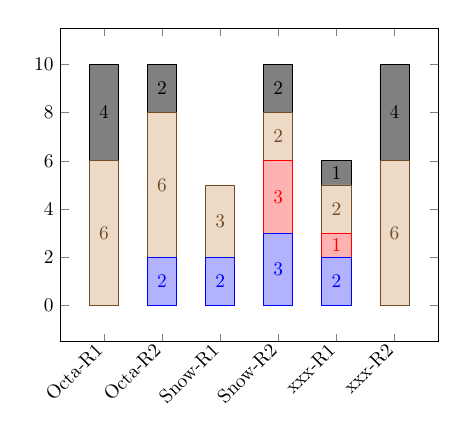
\begin{tikzpicture}[scale=0.7]
      \begin{axis}[
          ybar stacked,
	      bar width=15pt,
	      nodes near coords,
          enlargelimits=0.15,
          legend style={at={(0.5,-0.20)},
          anchor=north,legend columns=-1},
         % ylabel={\#Time (in ms)},
          symbolic x coords={Octa-R1, Octa-R2, Snow-R1, Snow-R2, 
	      xxx-R1, xxx-R2},
          xtick=data,
          x tick label style={rotate=45,anchor=east},
        ]
        \addplot+[ybar] plot coordinates {(Octa-R1,0) (Octa-R2,2) 
          (Snow-R1,2) (Snow-R2,3)  (xxx-R1,2) (xxx-R2,0)};
        \addplot+[ybar] plot coordinates {(Octa-R1,0) (Octa-R2,0) 
          (Snow-R1,0) (Snow-R2,3)  (xxx-R1,1) (xxx-R2,0)};
        \addplot+[ybar] plot coordinates {(Octa-R1,6) (Octa-R2,6)
          (Snow-R1,3) (Snow-R2,2) (xxx-R1,2) (xxx-R2,6)};
        \addplot+[ybar] plot coordinates {(Octa-R1,4) (Octa-R2,2) 
          (Snow-R1,0) (Snow-R2,2) (xxx-R1,1) (xxx-R2,4)};
       % \legend{\strut Geometry, \strut Curvature, \strut xx, \strut xx}
      \end{axis}
    \end{tikzpicture}
  \end{center}
  \caption{Adaptive timings H vs. rafined (tout : adaptatif, 2 rayons par formes, 4
    formes + images).}
  \label{fig:timings}
\end{figure}

\end{document}
